\documentclass[12pt]{article} % Документ принадлежит классу article, а также будет печататься в 12 пунктов.
\usepackage{array} % Для титульника
\usepackage{ucs}
\usepackage[utf8x]{inputenc} % Включаем поддержку UTF8
\usepackage[russian]{babel}  % Включаем пакет для поддержки русского языка
\usepackage[left=2cm,right=2cm, top=2cm,bottom=2cm,bindingoffset=0cm]{geometry} % Отступы по краям страницы
\usepackage{amssymb,amsfonts,amsmath,mathtext,cite,enumerate,float} % Математические штуки
\usepackage{cmap} % чтобы работал поиск по PDF
\usepackage{graphicx} % для вставки картинок

\usepackage{wrapfig} % Обтектание картинок текстом
 
%  для гиперссылок
\usepackage{xcolor}
\usepackage{hyperref}
\definecolor{linkcolor}{HTML}{191970} % цвет ссылок
\definecolor{urlcolor}{HTML}{191970} % цвет гиперссылок
\hypersetup{pdfstartview=FitH,  linkcolor=linkcolor,urlcolor=urlcolor, colorlinks=true}

\usepackage{pscyr} % Нормальные шрифты
\usepackage{setspace} % Для отступов между строк
%Это для формирования листингов
%%%%%%%%%%%%%%%%%%%%%%%%Листинги на MATLAB
\usepackage{listings}
\usepackage{color} %red, green, blue, yellow, cyan, magenta, black, white
\definecolor{mygreen}{RGB}{28,172,0} % color values Red, Green, Blue
\definecolor{mylilas}{RGB}{170,55,241}

\lstset{language=Matlab,
	breaklines=true,%
	morekeywords={matlab2tikz},
	keywordstyle=\color{blue},%
	morekeywords=[2]{1}, keywordstyle=[2]{\color{black}},
	identifierstyle=\color{black},%
	stringstyle=\color{mylilas},
	commentstyle=\color{mygreen},%
	showstringspaces=false,%without this there will be a symbol in the places where there is a space
	numbers=left,%
	numberstyle={\tiny \color{black}},% size of the numbers
	numbersep=9pt, % this defines how far the numbers are from the text
	emph=[1]{for,end,break},emphstyle=[1]\color{blue}, %some words to emphasise
	inputencoding=cp1251
	%emph=[2]{word1,word2}, emphstyle=[2]{style},    
}

%%%%%%%%%%%%%%%%%%%%%%%%%%%%%%%%%


\begin{document} % Начало документа

\title{{\large Распознавание образов. Лабораторная работа №2.} \\
	\textbf{\textquotedblleft Распознавание образов, описываемых гауссовскими случайными
	векторами\textquotedblright}.\\
	{\large Вариант 8 (а)}}
\date{}
\author{\textit{Выполнил}: студент 4 курса, группы 6.1 \\
	Суходолов Денис}
        
\maketitle

\begin{spacing}{1} % Для отступов между строк
\section*{Описание работы}
\textbf{Цель работы}: синтезировать алгоритмы распознавания образов,
описываемых  гауссовскими  случайными  векторами.  Исследовать
синтезированные алгоритмы распознавания с точки зрения ожидаемых потерь
и ошибок. Вычислить вероятности ошибок первого и второго рода на основе
выражений:
$$\alpha = \int\limits_{-\infty}^{l_0'}N(g'', m_{g_1},D_{g_1})dg'', \;\;\;\;\;\;\;\;\; \beta = \int\limits^{\infty}_{l_0'}N(g'', m_{g_2},D_{g_2})dg'' $$
\textbf{Ошибки первого рода} – при предъявлении образа одного класса, алгоритм классификации не относит образ к соответствующему классу (отвержение верной гипотезы).
~\\
\textbf{Ошибки второго рода}  – при предъявлении образа одного класса, алгоритм классификации относит образ к другому классу (принятие неверной гипотезы).
~\\
\textbf{Параметры}:
$$m_1\;=\;[2\;-3],\;m_2\;=\;[1\;10],\;C\;=\;[3\;-1;\;-1\;4],\;N_1\;=\;150, N_2\;=\;200$$
\section*{Программный код}
\lstinputlisting[basicstyle=\ttfamily\footnotesize ]{MyCoolLabFinal.m} 
\section*{Результат работы}
\begin{figure}[h]
	\begin{center}
		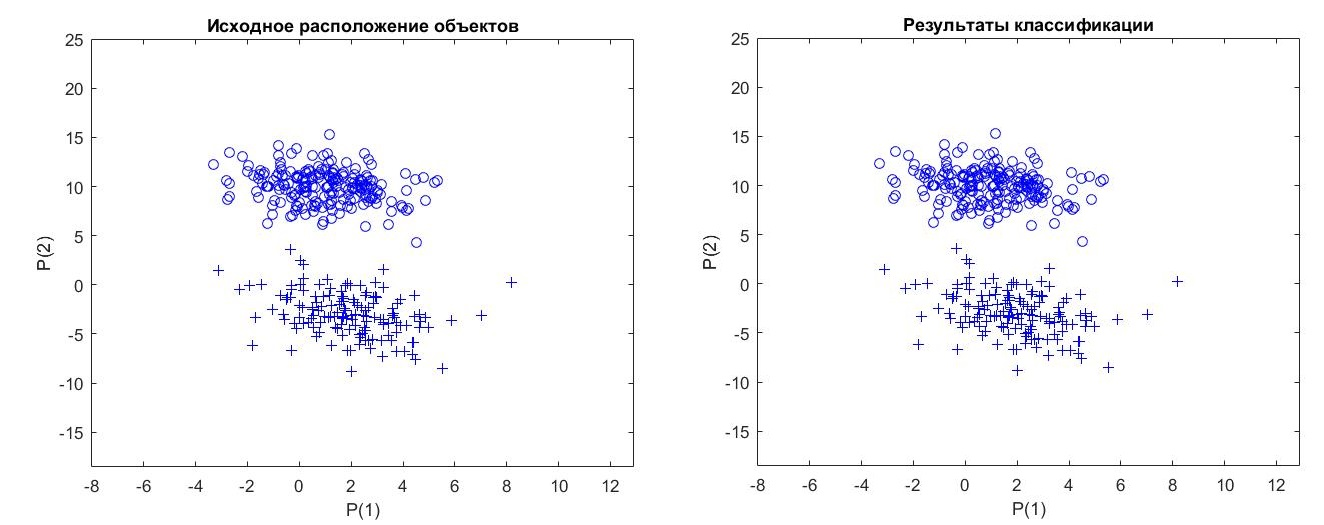
\includegraphics[width = 18cm]{1.jpg}
		%\caption{Результат работы алгоритма}
	\end{center}
\end{figure}
~\\
{\ttfamily\footnotesize 
alpha = 0.000525094 
~\\
beta = 0.00038498 }




\end{spacing}
\end{document}